\documentclass[]{article}
\usepackage{lmodern}
\usepackage{amssymb,amsmath}
\usepackage{ifxetex,ifluatex}
\usepackage{fixltx2e} % provides \textsubscript
\ifnum 0\ifxetex 1\fi\ifluatex 1\fi=0 % if pdftex
  \usepackage[T1]{fontenc}
  \usepackage[utf8]{inputenc}
\else % if luatex or xelatex
  \ifxetex
    \usepackage{mathspec}
    \usepackage{xltxtra,xunicode}
  \else
    \usepackage{fontspec}
  \fi
  \defaultfontfeatures{Mapping=tex-text,Scale=MatchLowercase}
  \newcommand{\euro}{€}
\fi
% use upquote if available, for straight quotes in verbatim environments
\IfFileExists{upquote.sty}{\usepackage{upquote}}{}
% use microtype if available
\IfFileExists{microtype.sty}{%
\usepackage{microtype}
\UseMicrotypeSet[protrusion]{basicmath} % disable protrusion for tt fonts
}{}
\usepackage[margin=1in]{geometry}
\usepackage{color}
\usepackage{fancyvrb}
\newcommand{\VerbBar}{|}
\newcommand{\VERB}{\Verb[commandchars=\\\{\}]}
\DefineVerbatimEnvironment{Highlighting}{Verbatim}{commandchars=\\\{\}}
% Add ',fontsize=\small' for more characters per line
\usepackage{framed}
\definecolor{shadecolor}{RGB}{248,248,248}
\newenvironment{Shaded}{\begin{snugshade}}{\end{snugshade}}
\newcommand{\KeywordTok}[1]{\textcolor[rgb]{0.13,0.29,0.53}{\textbf{{#1}}}}
\newcommand{\DataTypeTok}[1]{\textcolor[rgb]{0.13,0.29,0.53}{{#1}}}
\newcommand{\DecValTok}[1]{\textcolor[rgb]{0.00,0.00,0.81}{{#1}}}
\newcommand{\BaseNTok}[1]{\textcolor[rgb]{0.00,0.00,0.81}{{#1}}}
\newcommand{\FloatTok}[1]{\textcolor[rgb]{0.00,0.00,0.81}{{#1}}}
\newcommand{\CharTok}[1]{\textcolor[rgb]{0.31,0.60,0.02}{{#1}}}
\newcommand{\StringTok}[1]{\textcolor[rgb]{0.31,0.60,0.02}{{#1}}}
\newcommand{\CommentTok}[1]{\textcolor[rgb]{0.56,0.35,0.01}{\textit{{#1}}}}
\newcommand{\OtherTok}[1]{\textcolor[rgb]{0.56,0.35,0.01}{{#1}}}
\newcommand{\AlertTok}[1]{\textcolor[rgb]{0.94,0.16,0.16}{{#1}}}
\newcommand{\FunctionTok}[1]{\textcolor[rgb]{0.00,0.00,0.00}{{#1}}}
\newcommand{\RegionMarkerTok}[1]{{#1}}
\newcommand{\ErrorTok}[1]{\textbf{{#1}}}
\newcommand{\NormalTok}[1]{{#1}}
\usepackage{graphicx}
\makeatletter
\def\maxwidth{\ifdim\Gin@nat@width>\linewidth\linewidth\else\Gin@nat@width\fi}
\def\maxheight{\ifdim\Gin@nat@height>\textheight\textheight\else\Gin@nat@height\fi}
\makeatother
% Scale images if necessary, so that they will not overflow the page
% margins by default, and it is still possible to overwrite the defaults
% using explicit options in \includegraphics[width, height, ...]{}
\setkeys{Gin}{width=\maxwidth,height=\maxheight,keepaspectratio}
\ifxetex
  \usepackage[setpagesize=false, % page size defined by xetex
              unicode=false, % unicode breaks when used with xetex
              xetex]{hyperref}
\else
  \usepackage[unicode=true]{hyperref}
\fi
\hypersetup{breaklinks=true,
            bookmarks=true,
            pdfauthor={Heather E. Wheeler1,2, GTEx Consortium, Kaanan P. Shah3, . . ., Nancy J. Cox4, Dan L. Nicolae3, Hae Kyung Im3},
            pdftitle={An atlas of the genetic architecture of gene expression traits across the entire human body},
            colorlinks=true,
            citecolor=blue,
            urlcolor=blue,
            linkcolor=magenta,
            pdfborder={0 0 0}}
\urlstyle{same}  % don't use monospace font for urls
\setlength{\parindent}{0pt}
\setlength{\parskip}{6pt plus 2pt minus 1pt}
\setlength{\emergencystretch}{3em}  % prevent overfull lines
\setcounter{secnumdepth}{0}

%%% Use protect on footnotes to avoid problems with footnotes in titles
\let\rmarkdownfootnote\footnote%
\def\footnote{\protect\rmarkdownfootnote}

%%% Change title format to be more compact
\usepackage{titling}

% Create subtitle command for use in maketitle
\newcommand{\subtitle}[1]{
  \posttitle{
    \begin{center}\large#1\end{center}
    }
}

\setlength{\droptitle}{-2em}
%  \title{An atlas of the genetic architecture of gene expression traits across the entire human body}
  \title{Survey of Heritability and Sparsity of Gene Expression Traits across a Comprehensive Set of Human Tissues}
  \pretitle{\vspace{\droptitle}\centering\huge}
  \posttitle{\par}
  \author{Heather E. Wheeler\textsuperscript{1,2}, GTEx Consortium, Kaanan P.
Shah\textsuperscript{3}, . . ., Nancy J. Cox\textsuperscript{4}, Dan L.
Nicolae\textsuperscript{3}, Hae Kyung Im\textsuperscript{3}}
  \preauthor{\centering\large\emph}
  \postauthor{\par}
  \predate{\centering\large\emph}
  \postdate{\par}
  \date{\textsuperscript{1}Department of Biology and
\textsuperscript{2}Department of Computer Science, Loyola University
Chicago, \textsuperscript{3}Section of Genetic Medicine, Department of
Medicine, University of Chicago, \textsuperscript{4}Division of Genetic
Medicine, Vanderbilt University 2015-12-02 15:29:45}

\usepackage{setspace}
\setstretch{2}
\usepackage{soul}


\begin{document}

\maketitle

\section{Abstract}\label{abstract}

For most complex traits, gene regulation is known to play a crucial mechanistic role as demonstrated by the consistent enrichment of expression quantitative trait loci (eQTLs) among trait-associated variants. Thus, understanding of the genetic architecture of gene expression traits is key to elucidate the underlying mechanisms of complex traits. However, systematic survey of the heritability and the distribution of effect sizes across all representative tissues in the human body is not available.

Here we take advantage of the RNAseq data on a comprehensive set of tissue samples generated by the GTEx Consortium to fill this gap. We find that local h2 can be well characterized with xx\% of significant h2. However, the current sample sizes of ($<$400?) only allow us to compute distant h2 for a handful of genes (xx\% range). Bayesian Sparse Linear Mixed Model (BSLMM) estimates indicate that local architecture of gene expression traits is sparse rather than polygenic across all xx tissues examined.

To further delve into the tissue context specificity, we decompose the expression traits into cross tissue and tissue specific components. Heritability and sparsity estimates of these derived expression phenotypes show similar characteristics to the original traits. They also recapitulate complex Bayesian multi-tissue analysis results demonstrating that they reflect the expected biology. 

Finally, we apply this knowledge to develop prediction models of gene
expression traits for all tissues. The prediction models, heritability, and prediction performance R\textsuperscript{2} for original and (OTD-) derived phenotypes are made publicly available (\url{https://github.com/hakyimlab/PrediXcan}).


% For this reason, the GTEx project has generated RNA-Seq data
% on hundreds of individuals across more than 40 tissues providing a
% comprehensive atlas of gene expression traits.

% Here, we systematically
% examined the local versus distant heritability as well as the sparsity
% versus polygenicity of protein coding gene expression traits in tissues
% across the entire human body. To determine tissue context specificity,
% we decomposed the expression levels into cross-tissue and
% tissue-specific components via orthogonal tissue decomposition (OTD).
% Regardless of tissue type, we found that local heritability can be well
% characterized with current sample sizes. Unless strong functional priors
% are used, the heritability due to distant variants cannot be estimated.
% We also find that the distribution of effect sizes is more consistent
% with a sparse architecture across all tissues. We also show that the
% cross-tissue and tissue-specific expression phenotypes constructed with
% our OTD model recapitulate complex Bayesian multi-tissue analysis
% results demonstrating that they reflect the expected biology. Finally,
% this knowledge was applied to develop prediction models of gene
% expression traits for all tissues. The prediction models, heritability
% for each tissue, and prediction performance R\textsuperscript{2} are
% made publicly available (\url{https://github.com/hakyimlab/PrediXcan}).

\section{Introduction}\label{introduction}

\hl{using highlighted titles for main message - will delete all highlighted text in Intro when done}\\

\hl{gene regulation is important in genetic control of disease}
Regulatory variation plays a key role in the genetics of complex traits
{[}1--3{]}. 

\hl{why should we care about h2}

\hl{local h2. distal not well estimated. We don't solve this issue, so we should de-emphasize this.}

Most human expression quantitative trait loci (eQTL) studies
have focused on how local genetic variation affects gene expression in
order to reduce the multiple testing burden that would be required for a
global analysis {[}7,8{]}. Furthermore, when both local and distal eQTLs
are reported {[}9--11{]}, effect sizes and replicability are much higher
for local eQTLs. Indeed, while the heritability of gene expression
attributable to local genetic variation has been estimated accurately,
large standard errors have prevented accurate estimation of the
contribution of distal genetic variation to gene expression variation
{[}11,12{]}. However, an average contribution of distal heritability can be computed with accuracy when the estimates are allowed to be negative ]cite{alkes}. \hl{should we compute this? Alkes provides software to do that}

no published confidence intervals in h2 estimates

\hl{why should we care about sparsity, borrow ideas from Albert and Kruglyak}


\hl{polygenicity} While many common diseases have are likely polygenic
{[}4--6{]}, it is unclear whether gene expression levels are also
polygenic or instead have simpler genetic architectures. It is also
unclear how much these expression architectures vary across genes
{[}7{]}. 


\hl{prediction model performance indicated sparse rather than polygenic}

Prediction model performances can tell us a lot about the effect size distribution. When we developed whole blood expression prediction models we found that ...

We assessed the ability of various models, with different underlying
assumptions, to predict gene expression in order to both understand the
underlying genetic architecture of gene expression and to further
optimize predictors for our complex trait prediciton method, PrediXcan
{[}13{]}. In our PrediXcan paper, we showed that a polygenic score model
was suboptimal to more sparse models like the elastic net model with
\(\alpha=0.5\). However, a top eQTL only model did not do as well as the
elastic net either {[}13{]}, suggesting that for many genes, the genetic
architecture is sparse, but not regulated by one SNP. Gene expression
traits with sparse architecture should be better predicted with models
such as LASSO (Least Absolute Shrinkage and Selection Operator), which
prefers solutions with fewer parameters, each of large effect {[}14{]}.
Conversely, highly polygenic traits should be better predicted with
ridge regression or similarly polygenic models that prefer solutions
with many parameters, each of small effect {[}15--17{]}. 

\hl{here we verify this by computing the proportion of small effects to large effects using BSLMM across all tissues}

To obtain a
more thorough understanding of gene expression achitecture, we used the
hybrid approaches of the elastic net and BSLMM (Bayesian Sparse Linear
Mixed Model) {[}18{]} to quantify sparse and polygenic effects.

\hl{eqtl limited tissues until GTEx }

Most previous human eQTL studies were performed in whole blood or
lymphoblastoid cell lines due to ease of access or culturabilty
{[}9,19,20{]}. The Genotype-Tissue Expression (GTEx) Project aims to
examine the genetics of gene expression more comprehensively and
recently published a pilot analysis of eQTL data from 1641 samples
across 43 tissues from 175 individuals confirming that eQTLs are highly
shared across tissues {[}21{]}. We also showed that gene expression
predictors perform well across tissues {[}13{]}. 

\hl{OTD}

In order to harness
this cross-tissue effect for prediction and to better understand the
genetic architecture of tissue-specific and cross-tissue gene
regulation, we developed a mixed effects model called orthogonal tissue
decomposition (OTD) to determine the cross-tissue and tissue-specific
components of gene expression in the rich GTEx dataset. We modeled the
underlying genetic architecture of the cross-tissue and tissue-specific
gene expression components and developed predictors for use in PrediXcan
{[}13{]}.

\section{Results}\label{results}

\subsection{Local genetic variation can be well characterized for all
tissues}\label{local-genetic-variation-can-be-well-characterized-for-all-tissues}

\hl{local and distal h2 across tissues}

We estimated the local and distal heritability of gene expression levels in 40 tissues from the GTEx consortium and whole blood from the Depression Genes and Networks (DGN) cohort. The sample size in GTEx varied from xxx to xxx depending on the tissue and DGN had 922 samples {[}20{]}.
We used mixed-effects model (see Methods) and calculated variances using restricted maximum likelihood as implemented in GCTA {[}22{]}.

For the local component, we used variants within 1Mb of the TSS and TSE of each protein coding gene whereas for the distal component we used variants outside of the chromosome where the gene was located. See details in Methods. Different approaches to compute the distal genetic relatedness were explored but results did not change substantively.

The left column of Figure 1 shows the estimated local and distal h2 from DGN. Even though many genes show relatively large point estimates of distal h2, only the ones colored in blue are significantly different from zero. The local component of h2 is relatively well estimated in DGN with 52.6\% of genes  (xxx out of total xxx) showing h2 values significantly different from 0. In contrast, the distal heritability is significantly different from 0 for only 3.2\% (xxx out of xxx tested) of the genes. \hl{what are the denominators in these percentage calculations? All `expressed` genes in the tissue or all protein coding genes?}

\hl{TODO: generate table 1}

Table 1 summarizes the heritability estimate results across all tissues. It shows the mean h2 (\hl{this makes more sense if we use Alkes' method. If we use the GCTA we should clarify that it is biased because of the fact or not show it. We need to decide on this.}), mean se of h2 (local and distal), proportion of significant h2, number of significant genes, and number of expressed genes (definition? more than xx individuals with xx RPKM).

\hl{Relative contribution of local and distal variation to h2. Should we do this?}

% We fit
% two joint models, each with the same local genetic relationship matrix
% (GRM) and a two different distal GRMs. The local GRM was derived from
% SNPs within 1 Mb of each gene in both models. In model 1, the distal GRM
% was derived from all SNPs on non-gene chromosomes. In model 2, the
% distal GRM was derived from SNPs that are located on non-gene
% chromosomes and are eQTLs in the Framingham Heart Study (FHS) cohort
% (n=5257, FDR \textless{} 0.05) {[}23{]}.

% The mean local
% h\textsuperscript{2} was similar in both models, 0.123 in model 1 and
% 0.130 in model 2 (Fig 1). Of expressed genes, 52.6\% and 54.6\% had a
% positive 95\% confidence interval (CI) for the local estimate in models
% 1 and 2, respectively. The mean distal h\textsuperscript{2} was 0.123
% with a standard error (SE) of 0.284 in model 1, while the mean distal
% h\textsuperscript{2} was 0.076 with a SE of 0.142 in model 2. Using
% functional priors (known eQTLs) to define distal h\textsuperscript{2} in
% model 2 increased the percentage of genes with a positive CI from 3.2\%
% to 4.2\% (Fig 1). In model 2, the maximum local h\textsuperscript{2} was
% 0.93 with a standard error (SE) of 0.009 while the maximum distal
% h\textsuperscript{2} was 0.91 with a SE of 0.16.
%
% We also estimated the heritability of gene expression in the 9 tissues
% from the GTEx Project with the largest sample sizes, which ranged from
% 190-361 samples (see Methods). Mean local h\textsuperscript{2} estimates
% ranged from 0.028-0.044 with 4.4-8.6\% of genes having a positive CI
% (Fig 2). While the reduced sample sizes reduced the overall mean,
% maximum local h\textsuperscript{2} estimates in each tissue ranged from
% 0.79-0.91, similar to the maximum seen in DGN. As expected, distal
% h\textsuperscript{2} (eQTLs on non-gene chromosomes) could not be
% reliably estimated in these smaller sample sizes as less than 1\% of
% genes in each tissue had a positive CI in the joint model (Fig
% 3-\textbf{{[}SUP{]}})). Thus, we focus on the local architecture in
% subsequent sections.

Since it has been shown that local-eQTLs are more likely to be distal-eQTL, we tested whether restricting the distal genetic similarity computation to cis-eQTLs for other genes could improve distal heritability precision by prioritizing functional variants. We exclude eQTLs in the same chr as the tested gene to avoid contaminating distal h2 with cis associations. 

Using
functional priors (known eQTLs) to define distal h\textsuperscript{2} increased the percentage of genes with a positive CI from 3.2\%
to 4.2\% in whole blood (Fig 1). In GTEx tissues the increase ranged from xxx to xxx. \hl{TODO: do the same genes have signif h2? compare h2 and se from both estimates model1 vs model2}


\subsection{The effect of local genetic variation on gene expression is
sparse rather than
polygenic}\label{the-effect-of-local-genetic-variation-on-gene-expression-is-sparse-rather-than-polygenic}

\subsection{Sparse local architecture revealed by performance of prediction models}

We performed 10-fold cross-validation using the elastic net {[}24{]} to
test the predictive performance of local SNPs for gene expression across
a range of mixing parameters, \(\alpha\). The \(\alpha\) that gives the
largest cross-validation R\textsuperscript{2} informs the sparsity of
each gene expression trait. That is, at one extreme, if the optimal
\(\alpha=0\) (equivalent to ridge regression), the gene expression trait
is highly polygenic, whereas if the optimal \(\alpha=1\) (equivalent to
LASSO), the trait is highly sparse. We found that for most gene
expression traits, the cross-validated R\textsuperscript{2} was
suboptimal for \(\alpha=0\) and \(\alpha=0.05\), but nearly identically
optimal for \(\alpha=0.5\) through \(\alpha=1\) in the DGN cohort (Fig
4). An \(\alpha=0.05\) was also clearly suboptimal for gene expression
prediction in the nine GTEx tissues, while models with
\(\alpha=0.5,0.95,\) or 1 had similar predictive power (Fig
5-\textbf{{[}SUP{]}}). This suggests that for most genes, the effect of
local genetic variation on gene expression is sparse rather than
polygenic.

\subsection{direct estimation of sparsity}

To further validate this result, we turned to the BSLMM {[}18{]} approach, which models the genetic contribution as the sum of a sparse and a polygenic components. This allowed us to directly estimate the proportion of each component. The total variance explained (PVE) by additive genetic variants is Bayesian equivalent of the chip heritability we have estimated using a linear mixed model as implemented in GCTA. The proportion of the genetic variance explained by sparse effects (PGE) is a useful measure of sparsity. 

We find that when the sample size is large enough, such as in DGN, there is a strong correlation
between BSLMM-estimated PVE and GCTA-estimated h\textsuperscript{2} (Fig
6A, R=0.96). We also find that for high heritability genes, the sparse component is large.  
For example, all genes with
PVE \textgreater{} 0.50 had PGE \textgreater{} 0.82 and their median PGE
was 0.989 (Fig 6B). The median PGE for genes with PVE \textgreater{} 0.1
was 0.949. Fittingly, for most (96.3\%) of the genes with PVE estimates
\textgreater{} 0.10, the median number of SNPs included in the model was
no more than 10 (Fig 6C).

%To further validate this result, we used BSLMM {[}18{]} to
%define the total proportion of variance in expression explained by
%sparse and polygenic effects together (PVE) and the proportion of this
% genetic variance explained by sparse effects (PGE) for local SNPs in
% each gene in the DGN cohort. The PVE can be thought of as a Bayesian
% estimate of chip heritability and, indeed, there is a strong correlation
% between BSLMM-estimated PVE and GCTA-estimated h\textsuperscript{2} (Fig
% 6A, R=0.96). For genes with large PVE, the PGE also was large,
% indicative of a sparse genetic architecture. For example, all genes with
% PVE \textgreater{} 0.50 had PGE \textgreater{} 0.82 and their median PGE
% was 0.989 (Fig 6B). The median PGE for genes with PVE \textgreater{} 0.1
% was 0.949. Fittingly, for most (96.3\%) of the genes with PVE estimates
% \textgreater{} 0.10, the median number of SNPs included in the model was
% no more than 10 (Fig 6C).

Interestingly, when we applied BSLMM to the GTEx data, we found that
many genes had strikingly larger BSLMM-estimated PVE than GCTA-estimated
h\textsuperscript{2} (Fig 7). This likely reflects the increased power
of the BSLMM method at the lower sample sizes (\(n \leq 361\)) present
in GTEx to estimate variance explained when the trait is more sparse
than polygenic. GCTA assumes an underlying polygenic model, but as we
saw in DGN, BSLMM-estimated PVE and GCTA-estimated h\textsuperscript{2}
are more correlated when the sample size is larger (n=922, Fig 6A). As
we observed in DGN, genes with larger PVE estimates were more likely to
have a PGE estimate approaching 1 with a lower credible set greater than
0.01 in each of the nine GTEx tissues (Fig 8).

\subsection{Cross-tissue and tissue specific decomposition}

Since a substantial portion of local regulation was shown to be common across multiple tissues, we sought to decompose the expression levels into a component that is common across all tissues and a tissue specific components. For this we used a linear mixed effects models as described in the Methods section. We call this approach orthogonal tissue decomposition (OTD) because the cross tissue and tissue specific components are assumed to be independent in the model.

The decomposition is applied at the expression trait level so that the downstream genetic regulation analysis is performed separately for each one. This simplifies computation.\hl{reword this last sentence}

\subsection{Cross-tissue expression phenotype has increased predictive
power and recapitulates known multi-tissue eQTL target
genes}\label{cross-tissue-expression-phenotype-has-increased-predictive-power-and-recapitulates-known-multi-tissue-eqtl-target-genes}

% Using a marginal
% model with just the local GRM, we estimated the local
% h\textsuperscript{2} of cross-tissue gene expression and tissue-specific
% gene expression in the nine tissues with the most samples.

We compute the local heritability of these derived expression traits. 

The precision of the estimated h2 of the cross tissue h2 improves greatly compared to the estimates of each tissue. 

The
cross-tissue heritabilities were larger and the standard errors were
smaller than the tissue-specific estimates (Fig 9-\textbf{{[}SUP{]}}).
The percentage of GCTA h\textsuperscript{2} estimates with positive CIs
was much larger for cross-tissue expression (17.3\%) than the
tissue-specific expressions (all less than 3\%, Fig 10). Similarly, the
percentage of BSLMM PVE estimates with a lower credible set greater than
0.01 was 49\% for cross-tissue expression, but ranged from 24-27\% for
tissue-specific expression (Fig 11).

We also compared the cross-tissue h\textsuperscript{2} from the OTD to
h\textsuperscript{2} estimates from the pre-OTD measures of gene
expression in each of the nine tissues, which we term whole tissue
expression. Again, the cross-tissue heritabilities were larger and the
standard errors were smaller than the whole tissue estimates (Fig
12-\textbf{{[}SUP{]}}), though less striking than the tissue-specific
comparison. The percentage of whole tissue h\textsuperscript{2}
estimates with positive CIs ranged from 4.4-8.6\% and thus were all
larger than the tissue-specific postive CI percentages, but smaller than
the cross-tissue percentage (Fig 2). Cross-tissue BSLMM PVE estimates
had lower error than whole tissue PVE (Fig 8, Fig 11). Like whole tissue
expression, cross-tissue and tissue-specific expression showed better
predictive performance using the elastic-net when \(\alpha \geq 0.5\)
than when \(\alpha=0.05\) (Fig 13-\textbf{{[}SUP{]}}). Cross-tissue
predictive performance exceeded that of both tissue-specific and whole
tissue expression as indicated by higher cross-validated
R\textsuperscript{2} (Fig 5-\textbf{{[}SUP{]}}, Fig
13-\textbf{{[}SUP{]}}).

We compared our OTD results to those from a joint multi-tissue eQTL
analysis method {[}25{]}, which was previously performed on a subset of
the GTEx data {[}21{]}. The results of this analysis include eQTL
posterior probabilities for each of the nine tissues, which can be
interpreted as the probability a SNP is an eQTL in tissue \emph{x} given
the data. Using the top eQTL for each gene, we defined an entropy
statistic (see Methods) that combines the nine posterior probabilities
into one value such that higher entropy values mean the gene is more
likely to be regulated by the same eQTL across all nine tissues, rather
than in just a subset of the nine. We observed a strong correlation
between entropy and both the cross-tissue expression heritability (R =
0.082, Fig 14A) and PVE (R = 0.12, Fig 14B) estimates, using the
cross-tissue expression derived from the OTD. Thus, genes with high
cross-tissue heritability are more likely to have cross-tissue eQTLs,
confirming that OTD is capturing the cross-tissue component of gene
expression. Also, the correlation between tissue-specific OTD gene
expression PVE and the posterior probability that the gene has an eQTL
in that tissue is strongest in each respective tissue, confirming that
OTD also captures tissue-specific components of gene expression (Fig
15).

\section{Discussion}\label{discussion}

Because regulatory variation plays a key mechanistic role in the
genetics of complex traits {[}1--3{]}, we sought to comprehensively
characterize the genetic architecture of gene expression across tissues.
We accurately quantify the local heritability of gene expression in DGN
whole blood and nine GTEx tissues. In DGN, the mean local
h\textsuperscript{2} was 0.13, similar to that found in family studies
of blood expression, where mean h\textsuperscript{2} ranged from
0.07-0.11 {[}11,12{]}. While we found that functional priors (known
trans-eQTLs) can reduce the error of the estimate by reducing the number
of genetic markers included in the genetic relationship matrix, larger
sample sizes (n \textgreater{} 1000) are needed to accurately estimate
distal heritability.

Using the hybrid polygenic-sparse approach of BSLMM (Bayesian Sparse
Linear Mixed Model) {[}18{]}, we show that the local architecture of
gene expression is sparse (high PGE) for most heritable genes in both
DGN and GTEx. Using the elastic net {[}24{]}, we observed improved
cross-validated expression prediction for \(\alpha \geq 0.5\) across
tissues, confirming the sparsity result. This result demonstrates that
sparse effects can be identified with sample sizes in the hundreds
rather than the thousands and is supported by many prior studies with
sample sizes near 100 that identified replicable eQTLs near the
transcription start sites of genes{[}9{]}. Conversely, for traits that
are highly polygenic, e.g.~height, BMI, schizophrenia, and bipolar
disorder, thousands to tens of thousands of samples are needed to
identify significant genetic signals {[}26{]}. Therefore, the distal
contributions to expression h\textsuperscript{2} are likely to be more
polygenic because they could not be accurately estimated here with
sample sizes in the hundreds.

Our BSLMM analysis quantified the optimal number of SNPs to include for
each gene. For example, the median number of SNPs for \emph{ERAP2} was
1. When we previously plotted out-of-sample observed vs.~predicted
expression using elastic net (\(\alpha=0.5\)) generated predictors for
this gene, we saw three clusters, corresponding to each of the three
genotypes for the causal variant {[}13{]}. Similarly, BSLMM estimated 2,
3, and 5 SNPs for \emph{PEX6}, \emph{NUDT2}, and \emph{ERAP1},
respectively, consistent with the out-of-sample observed vs.~predicted
expression plots in our PrediXcan paper (see Figure 5 in {[}13{]}).
Potentially due to variations in imputation quality of the input SNPs
for expression prediction, it is useful to include more than the likely
causal variants (i.e.~elastic net rather than BSLMM) in the prediction
for robustness. In addition, the elastic net is amenable
cross-validation, while genome-wide cross-validation with BSLMM is
impractical at current runtimes.

We developed a mixed effects model called orthogonal tissue
decomposition (OTD) to determine the cross-tissue and tissue-specific
components of gene expression in the GTEx dataset. Previous studys have
shown that many eQTLs are shared across tissues {[}21,25{]}. In
addition, because expression data from multiple tissues were available
from the same individuals in GTEx, we could effectively use the multiple
tissue samples as subject replicates in our OTD model. However, the
tissue availability is unbalanced across individuals because of the
difficulties of sample collection and the uneven quality of the tissues.
By combining all available expression data in our OTD model, we found
that estimates of the local heritability of cross-tissue gene expression
have larger magnitude and improved standard errors compared to single
tissue estimates due to the borrowing of information across all samples.
Thus, OTD effectively increases power to estimate heritability.
Comparing our OTD results to a previously performed joint multi-tissue
eQTL analysis method {[}25{]}, we show that genes with high cross-tissue
heritability are more likely to have cross-tissue eQTLs, confirming that
OTD is capturing the cross-tissue component of gene expression.

We confirmed that OTD also captures tissue-specific components of gene
expression by showing the correlation between tissue-specific OTD gene
expression PVE and the posterior probability that the gene has an eQTL
in that tissue is strongest in each respective tissue. Interestingly,
whole blood and thyroid appear to be outliers in that they each have a
negative correlation with all the other tissues (Fig 15). In the GTEx
pilot analysis, whole blood had the lowest levels of eQTL sharing with
other tissues and thyroid had the largest number of cis-eQTL genes,
which implies a higher number of tissue-specific eQTLs {[}21{]}.

In this paper, we quantitate the genetic architecture of gene expression
and develop predictors across tissues. We show that local heritability
can be accurately estimated across tissues, but distal heritability
cannot be reliably estimated at current sample sizes. Using two
different approaches, the elastic net and BSLMM, we show that for local
gene regulation, the genetic architecture is mostly sparse rather than
polygenic. Using new expression phenotypes generated in our OTD model,
we show that cross-tissue predictive performance exceeded that of both
tissue-specific and whole tissue expression as indicated by higher
elastic net cross-validated R\textsuperscript{2}. Predictors generated
in this study of gene expression architecture have been added to our
PrediXcan database (\url{https://github.com/hakyimlab/PrediXcan})
{[}13{]} for use in future studies of complex trait genetics.

\section{Methods}\label{methods}

\subsection{Genomic and Transcriptomic
Data}\label{genomic-and-transcriptomic-data}

\subsubsection{DGN Dataset}\label{dgn-dataset}

We obtained whole blood RNA-Seq and genome-wide genotype data for 922
individuals from the Depression Genes and Networks (DGN) cohort
{[}20{]}, all of European ancestry. For our analyses, we used the HCP
(hidden covariates with prior) normalized gene-level expression data
used for the \emph{trans}-eQTL analysis in Battle et al. {[}20{]} and
downloaded from the NIMH repository. The 922 individuals were unrelated
(all pairwise \(\hat{\pi}\) \textless{} 0.05) and thus all included in
downstream analyses. Imputation of approximately 650K input SNPs (minor
allele frequency {[}MAF{]} \textgreater{} 0.05, Hardy-Weinberg
Equilibrium {[}P \textgreater{} 0.05{]}, non-ambiguous strand {[}no A/T
or C/G SNPs{]}) was performed on the University of Michigan
Imputation-Server
(\url{https://imputationserver.sph.umich.edu/start.html}) {[}27,28{]}
with the following parameters: 1000G Phase 1 v3 ShapeIt2 (no singletons)
reference panel, SHAPEIT phasing, and EUR population. Approximately 1.9M
non-ambiguous strand SNPs with MAF \textgreater{} 0.05, imputation
R\textsuperscript{2} \textgreater{} 0.8 and, to reduce computational
burden, inclusion in HapMap Phase II were retained for subsequent
analyses.

\subsubsection{GTEx Dataset}\label{gtex-dataset}

We obtained RNA-Seq gene expression levels from 8555 tissue samples (53
unique tissue types) from 544 unique subjects in the GTEx Project
{[}21{]} data release on 2014-06-13. Of the individuals with gene
expression data, genome-wide genotypes (imputed with 1000 Genomes) were
available for 450 individuals. While all 8555 tissue samples were used
in the OTD model (described below) to generate cross-tissue and
tissue-specific components of gene expression, we used the nine tissues
with the largest sample sizes when quantifying tissue-specific effects.
Tissues and sample sizes (both RNA-seq and genotypes available) included
cross-tissue (\(n=450\)), skeletal muscle (\(n=361\)), whole blood
(\(n=339\)), skin from the sun-exposed portion of the lower leg
(\(n=303\)), subcutaneous adipose (\(n=298\)), tibial artery
(\(n=285\)), lung (\(n=279\)), thyroid (\(n=279\)), tibial nerve
(\(n=256\)) and left ventricle heart (\(n=190\)). Approximately 2.6M
non-ambiguous strand SNPs included in HapMap Phase II were retained for
subsequent analyses.

\subsection{Partitioning local and distal heritability of gene
expression}\label{partitioning-local-and-distal-heritability-of-gene-expression}

To investigate the proximity of gene expression regulation to each gene,
we partitioned the proportion of gene expression variance explained by
SNPs in the DGN cohort into two components: local (SNPs within 1Mb of
the gene) and distal (eQTLs on non-gene chromosomes) as defined by the
GENCODE {[}29{]} version 12 gene annotation. We calculated the
proportion of the variance (narrow-sense heritability) explained by each
component using the following mixed-effects model:

\[ Y_g = \sum_{k = \in local}w_{k,g} X_k + \sum_{k = \in distal}w_{k,g} X_k + \epsilon \]

Assuming a random effects for \(w_{k,g} \approx N(0, \sigma^2_w)\) and
\(\epsilon \approx N(0, \sigma^2_{\epsilon} I_n)\), where \(I_n\) is the
identity matrix, we calculated the total variability explained by local
and distal components by estimating \(\sigma^2_w\) with restricted
maximum likelihood (REML) using GCTA software {[}22{]}. For heritability
analyses in the GTEx cohort, we removed the \(distal\) term from the
model and only estimated marginal \(local\) h\textsuperscript{2} due to
the smaller sample sizes of both cross-tissue and tissue-specific
expression levels compared to DGN.

\subsection{Determining polygenicity versus sparsity using the elastic
net}\label{determining-polygenicity-versus-sparsity-using-the-elastic-net}

We applied the elastic net {[}24{]} to model the effect of local genetic
variation (SNPs within 1 Mb of gene) on the genetic architecture of gene
expression. We used the \texttt{cv.glmnet} function in the R package
\texttt{glmnet} {[}30,31{]} to perform 10-fold cross-validation of the
elastic net across a range of mixing paramaters (\(\alpha\)) to find the
\(\alpha\) that maximized predictive performance, measured by Pearson's
R\textsuperscript{2}. Specifically, \texttt{glmnet} solves the following
problem:

\textbf{{[}{[}Haky, should/can we simplify this equation? I just took it
from \url{http://web.stanford.edu/~hastie/glmnet/glmnet_alpha.html}, but
they don't explain all the terms{]}{]}}
{\[\min_{\beta_0,\beta} \frac{1}{N} \sum_{i=1}^{N} w_i l(y_i,\beta_0+\beta^T x_i) + \lambda\left[(1-\alpha)||\beta||_2^2/2 + \alpha ||\beta||_1\right], \]}

over a grid of values of \(\lambda\) covering the entire range
{[}30,31{]}. This tuning parameter \(\lambda\) controls the overall
strength of the penalty.

The elastic net penalty is controlled by mixing parameter \(\alpha\),
which spans LASSO (\(\alpha=1\), the default) {[}14{]} at one extreme
and ridge regression (\(\alpha=0\)) {[}15{]} at the other. The ridge
penalty shrinks the coefficients of correlated SNPs towards each other,
while the LASSO tends to pick one of the correlated SNPs and discard the
others. Thus, an optimal prediction R\textsuperscript{2} for
\(\alpha=0\) means the gene expression trait is highly polygenic, while
an optimal prediction R\textsuperscript{2} for \(\alpha=1\) means the
trait is highly sparse. An optimal prediction R\textsuperscript{2} in
between (e.g. \(\alpha=0.5\)) means the trait has a mixed genetic
architecture.

In the DGN cohort, we tested 21 values of the mixing parameter
(\(\alpha=0, 0.05, 0.1, ..., 0.90, 0.95, 1\)) for optimal prediction of
gene expression of the 341 genes on chromosome 22. For the rest of the
autosomes in DGN and for whole tissue, cross-tissue, and tissue-specific
expression in the GTEx cohort, we tested \(\alpha=0.05, 0.5, 0.95, 1\).

\subsection{Quantifying sparsity with Bayesian Sparse Linear Mixed
Models
(BSLMM)}\label{quantifying-sparsity-with-bayesian-sparse-linear-mixed-models-bslmm}

We used BSLMM {[}18{]} to model the effect of local genetic variation
(SNPs within 1 Mb of gene) on the genetic architecture of gene
expression. The BSLMM consists of a standard linear mixed model, with
one random effect term, and with sparsity inducing priors on the
regression coefficients {[}18{]}. We used the software GEMMA {[}32{]} to
implement BSLMM for each gene using the following parameters:

\begin{Shaded}
\begin{Highlighting}[]
\NormalTok{gemma -g [localGenoFile] -p [geneExpFile] -a [snpAnnotFile] -bslmm }\DecValTok{1} \NormalTok{-s }\DecValTok{100000} \NormalTok{-o [outFile]}
\end{Highlighting}
\end{Shaded}

The \texttt{-bslmm 1} option specifies a linear BSLMM and the
\texttt{-s 100000} option specifies the number of sampling steps per
gene. The BSLMM estimates the PVE (the total proportion of variance in
phenotype explained by the sparse effects and random effects terms
together) and PGE (the proportion of genetic variance explained by the
sparse effects terms). From the second half of the sampling iterations
for each gene, we report the median and the 95\% credible sets of the
PVE, PGE, and the \textbar{}\(\gamma\)\textbar{} parameter (the number
of SNPs with non-zero coefficients).

\subsection{Orthogonal tissue
decomposition}\label{orthogonal-tissue-decomposition}

To better understand the context specificity of gene expression
regulation, we developed a method called orthogonal tissue decomposition
(OTD). This approach is an extension of our method to develop an
intrinsic growth phenotype {[}33{]}. We applied OTD to GTEx Project
{[}21{]} data and decomposed the expression of each gene into
cross-tissue and tissue-specific components. The tissue availability is
unbalanced across individuals because of the difficulties of sample
collection and the uneven quality of the tissues. OTD decomposes the
expression traits into orthogonal components as represented by the
following model:

\[ Y_i = T_{i,cross} + T_{i,tissue} \]

Specifically, to generate cross-tissue and tissue-specific expression
levels, we used the \texttt{lmer} function in the R {[}34{]} package
\texttt{lme4} {[}35,36{]} to fit the following mixed-effects model:

\begin{Shaded}
\begin{Highlighting}[]
\NormalTok{fit <-}\StringTok{ }\NormalTok{lme4::}\KeywordTok{lmer}\NormalTok{(expression ~}\StringTok{ }\NormalTok{(}\DecValTok{1}\NormalTok{|SUBJID) +}\StringTok{ }\NormalTok{TISSUE +}\StringTok{ }\NormalTok{GENDER +}\StringTok{ }\NormalTok{PEERs)}
\end{Highlighting}
\end{Shaded}

The model included whole tissue gene expression levels in 8555 GTEx
tissue samples from 544 unique subjects. A total of 17,647
Protein-coding genes (defined by GENCODE {[}29{]} version 18) with a
mean gene expression level across tissues greater than 0.1 RPKM (reads
per kilobase of transcript per million reads mapped) were included in
the model. \texttt{SUBJID} was a random effect and the covariates
\texttt{TISSUE}, \texttt{GENDER}, and \texttt{PEERs} were fixed effects
used to predict whole tissue expression levels (\texttt{expression} in
the model). \texttt{PEERs} included the top 15 PEER factors estimated
across all tissues using the R package \texttt{PEER} {[}37{]} to control
for batch effects and experimental confounders. Cross-tissue expression
was defined as the random effects from the model (\texttt{ranef(fit)})
and tissue-specific expression as the residuals (\texttt{resid(fit})).

\subsection{Comparison of OTD PVE to multi-tissue eQTL
results}\label{comparison-of-otd-pve-to-multi-tissue-eqtl-results}

Using results from a joint multi-tissue eQTL analysis method {[}25{]}
performed with a subset of the GTEx data (maximum n=175 in the nine
tissues of the pilot phase, see {[}21{]}), we defined an entropy
statistic to compare these results to those from our OTD method. The
results of the multi-tissue analysis include eQTL posterior
probabilities for each of the nine tissues, which can be interpreted as
the probability a SNP is an eQTL in tissue \(t\) given the data. Using
the top eQTL for each gene \(g\), we defined the entropy \(S_g\) as:

\[ S_g = -\sum_{t}p_{t,g} \log p_{t,g} \]

where \(p_{t,g}\) is the eQTL probability in tissue \(t\) normalized to
1 for each gene \(g\). Thus, eQTLs with higher entropy statistics are
more likely to be cross-tissue eQTLs, rather than only regulating gene
expression in one or a few tissues. We calculated the Pearson
correlation between \(S_g\) and the cross-tissue expression heritability
and PVE for each gene to verify that our OTD method captures
cross-tissue effects. We also calculated a Pearson correlation matrix
between the posterior probabilities in each tissue from the multi-tissue
eQTL method and the tissue-specific gene expression PVE from the OTD
method.

\section{Figures}\label{figures}

\begin{figure}[htbp]
\centering
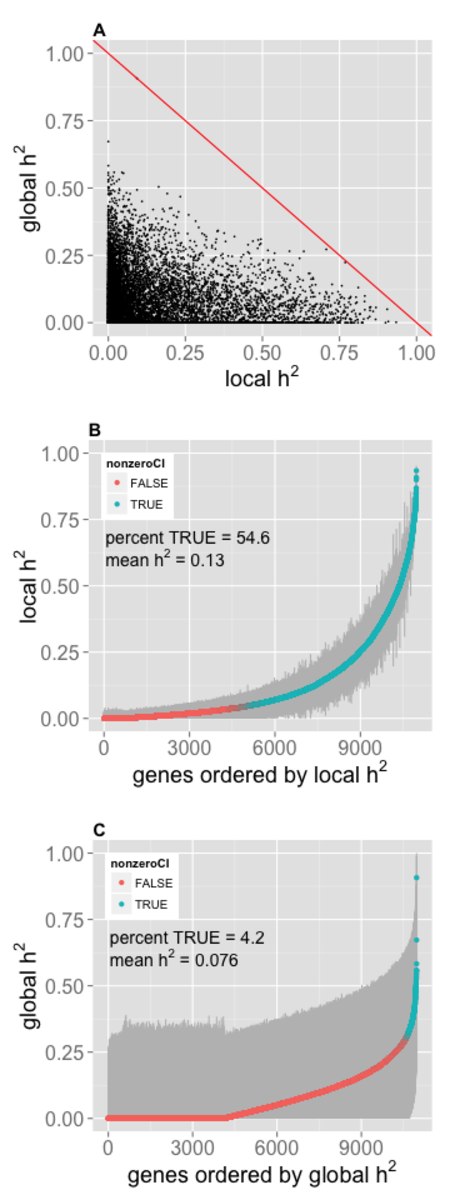
\includegraphics{GenArch_manuscript_files/figure-latex/jointH2-1.pdf}
\caption{DGN whole blood expression joint heritability
(h\textsuperscript{2}). Local (SNPs within 1 Mb of each gene) and distal
(Left: SNPs on non-gene chromsomes. Right: SNPs that are eQTLs in the
Framingham Heart Study on other chromosomes {[}FDR \textless{} 0.05{]})
h\textsuperscript{2} for gene expression were jointly estimated.
(\textbf{Top}) Distal h\textsuperscript{2} compared to local
h\textsuperscript{2} per gene in each model. (\textbf{Middle}) Local and
(\textbf{Bottom}) distal gene expression h\textsuperscript{2} estimates
ordered by increasing h\textsuperscript{2}. The 95\% confidence interval
(CI) of each h\textsuperscript{2} estimate is in gray and genes with a
lower bound greater than zero are in blue.}
\end{figure}

\begin{figure}[htbp]
\centering
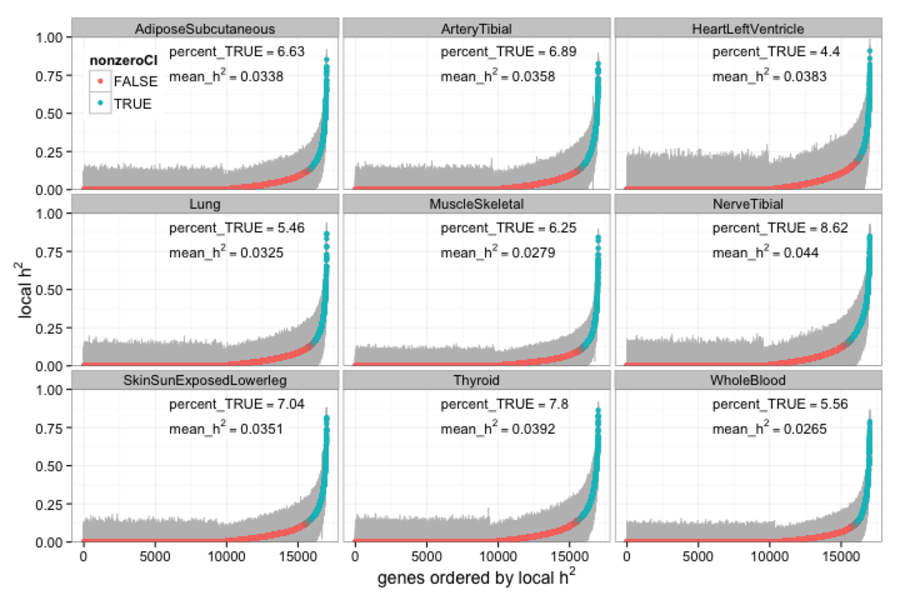
\includegraphics{GenArch_manuscript_files/figure-latex/TWlocalh2-1.pdf}
\caption{GTEx whole tissue local heritability (h\textsuperscript{2})
estimation. Local (SNPs within 1 Mb of each gene) gene expression
h\textsuperscript{2} estimates ordered by increasing
h\textsuperscript{2}. The 95\% confidence interval (CI) of each
h\textsuperscript{2} estimate is in gray and genes with a lower bound
greater than zero are in blue}
\end{figure}

\begin{figure}[htbp]
\centering
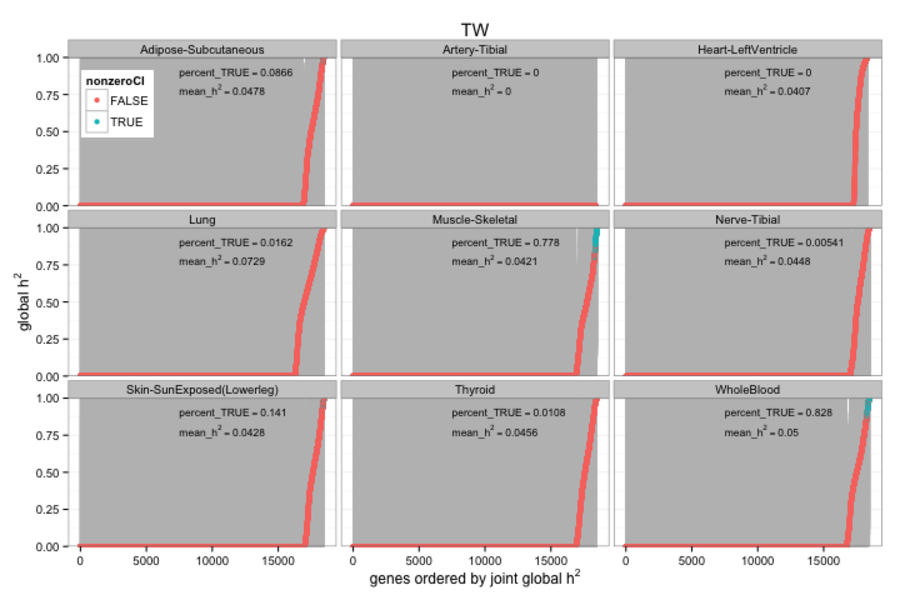
\includegraphics{GenArch_manuscript_files/figure-latex/TWglojth2-1.pdf}
\caption{GTEx whole tissue distal heritability (h\textsuperscript{2})
estimation. Distal (SNPs that are eQTLs in the Framingham Heart Study on
other chromosomes {[}FDR \textless{} 0.05{]}) gene expression
h\textsuperscript{2} estimates from a joint model are ordered by
increasing h\textsuperscript{2}. The 95\% confidence interval (CI) of
each h\textsuperscript{2} estimate is in gray and genes with a lower
bound greater than zero are in blue}
\end{figure}

\begin{figure}[htbp]
\centering
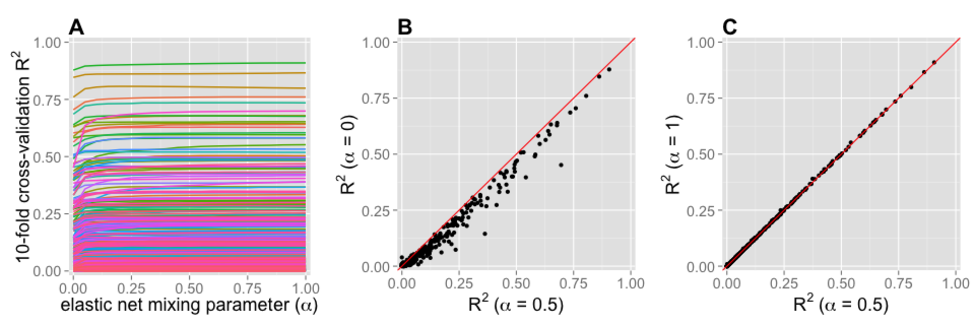
\includegraphics{GenArch_manuscript_files/figure-latex/EN-1.pdf}
\caption{DGN cross-validated predictive performance across the elastic
net. (\textbf{A}) 10-fold cross-validated R\textsuperscript{2} of
predicted vs.~observed expression in DGN whole blood compared to a range
of elastic net mixing parameters (\(\alpha\)) for genes on chromosome 22
with R\textsuperscript{2} \textgreater{} 0.3. (\textbf{B}) Predictive
R\textsuperscript{2} difference between LASSO (\(\alpha = 1\)) and
several other values of \(\alpha\) compared to LASSO predictive
R\textsuperscript{2} for 13171 autosomal genes.}
\end{figure}

\begin{figure}[htbp]
\centering
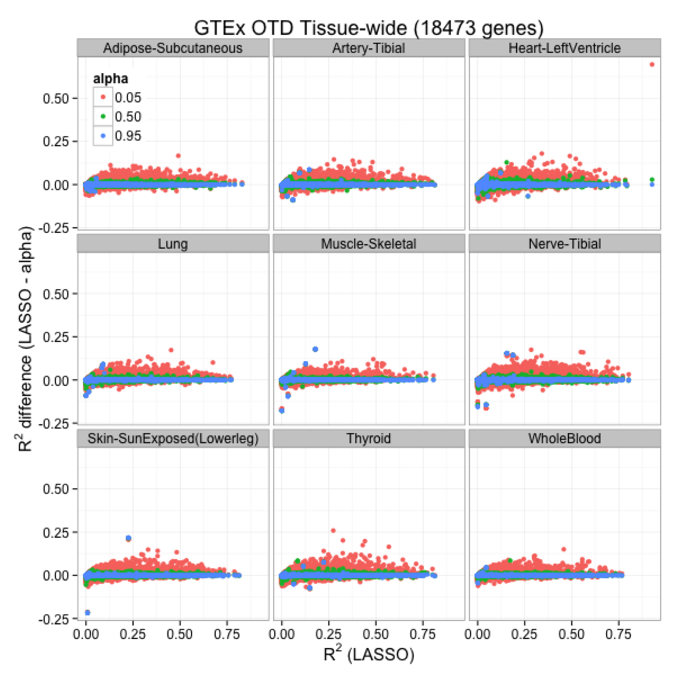
\includegraphics{GenArch_manuscript_files/figure-latex/ENtw-1.pdf}
\caption{GTEx whole tissue cross-validated predictive performance across
the elastic net. Predictive R\textsuperscript{2} difference between
LASSO (\(\alpha = 1\)) and several other values of \(\alpha\) compared
to LASSO predictive R\textsuperscript{2} for 18473 autosomal genes per
tissue.}
\end{figure}

\begin{figure}[htbp]
\centering
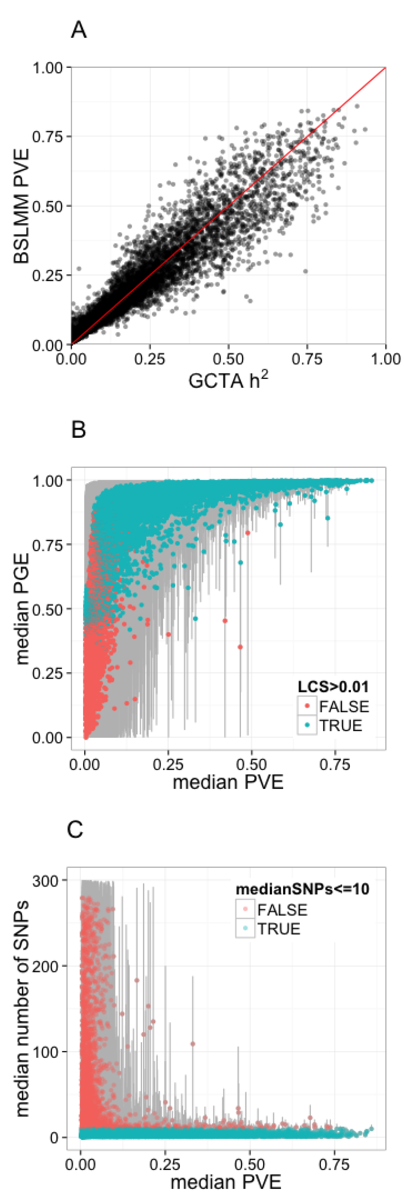
\includegraphics{GenArch_manuscript_files/figure-latex/dgnBSLMM-1.pdf}
\caption{Bayesian Sparse Linear Mixed Models reveal the sparsity of gene
expression architecture. (\textbf{A}) BSLMM-estimated PVE (total
proportion of variance explained) compared to GCTA-estimated
heritability per gene (R=0.96) (\textbf{B}) Comparison of median PGE
(proportion of PVE explained by sparse effects) to median PVE (total
proportion of variance explained) for expression of each gene. The 95\%
credible set of each PGE estimate is in gray and genes with a lower
credible set (LCS) greater than 0.01 are in blue. (\textbf{C})
Comparison of the median number of SNPs included in the model of each
gene to median PVE. The 95\% credible set of each SNP-number estimate is
in gray and genes with a median of 10 or fewer SNPs are in blue.}
\end{figure}

\begin{figure}[htbp]
\centering
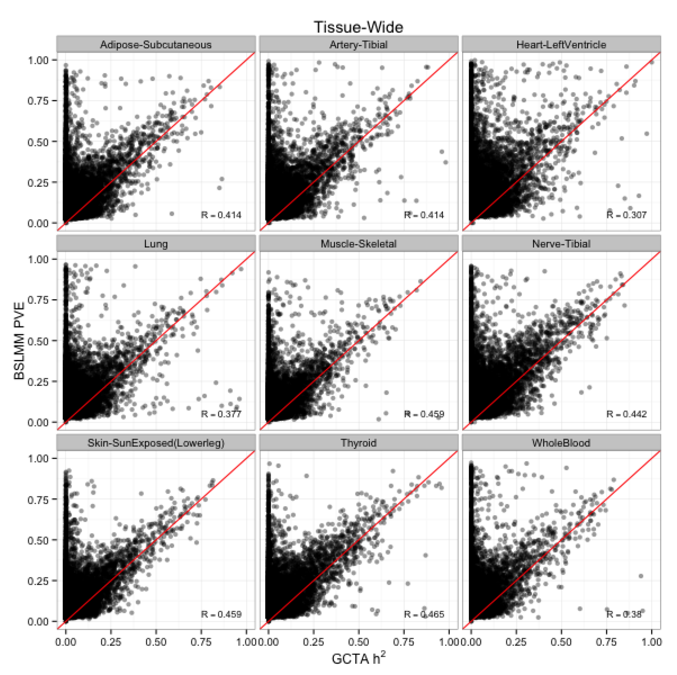
\includegraphics{GenArch_manuscript_files/figure-latex/TWpveh2-1.pdf}
\caption{GTEx whole tissue expression BSLMM-estimated PVE (total
proportion of variance explained) compared to GCTA-estimated
heritability per gene. R = Pearson correlation.}
\end{figure}

\begin{figure}[htbp]
\centering
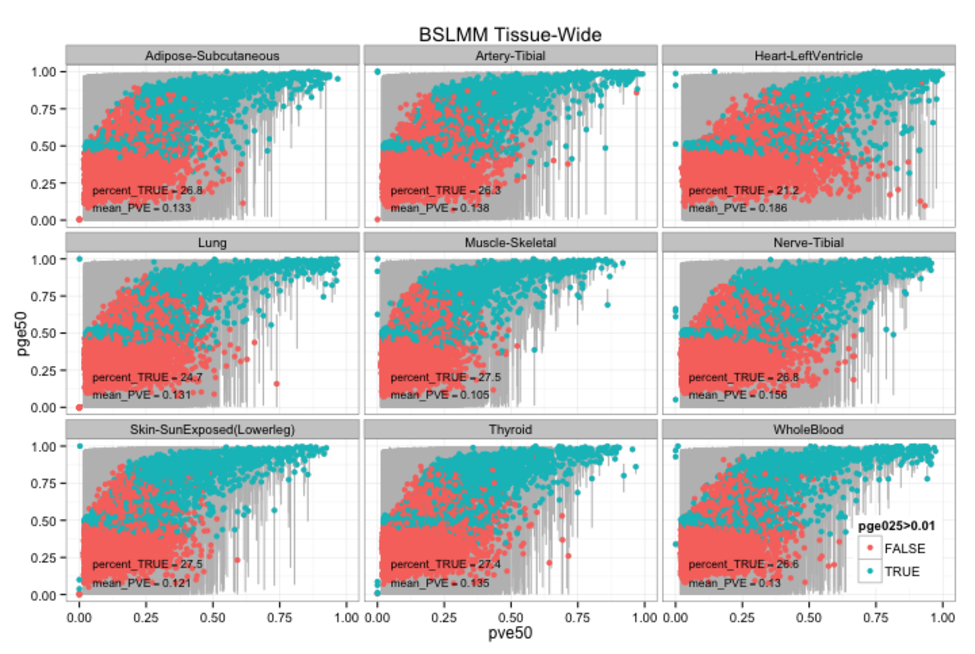
\includegraphics{GenArch_manuscript_files/figure-latex/TWbslmm-1.pdf}
\caption{GTEx whole tissue expression comparison of median PGE
(proportion of PVE explained by sparse effects) to median PVE (total
proportion of variance explained) for expression of each gene. The 95\%
credible set of each PGE estimate is in gray and genes with a lower
credible set (LCS) greater than 0.01 are in blue.}
\end{figure}

\begin{figure}[htbp]
\centering
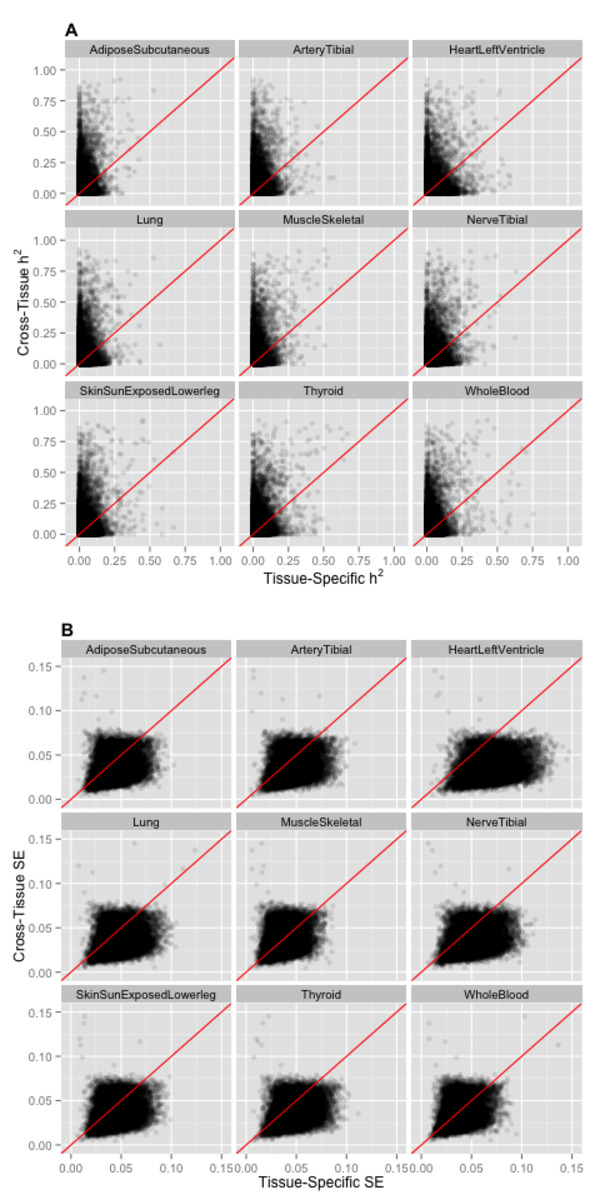
\includegraphics{GenArch_manuscript_files/figure-latex/TSotdH2SE-1.pdf}
\caption{Cross-tissue and tissue-specific comparison of heritability
(h\textsuperscript{2}, \textbf{A}) and standard error (SE, \textbf{B})
estimation. Cross-tissue local h\textsuperscript{2} is estimated using
the cross-tissue component (random effects) of the mixed effects model
for gene expression and SNPs within 1 Mb of each gene. Tissue-specifc
local h\textsuperscript{2} is estimated using the tissue-specific
component (residuals) of the mixed effects model for gene expression for
each respective tissue and SNPs within 1 Mb of each gene.}
\end{figure}

\begin{figure}[htbp]
\centering
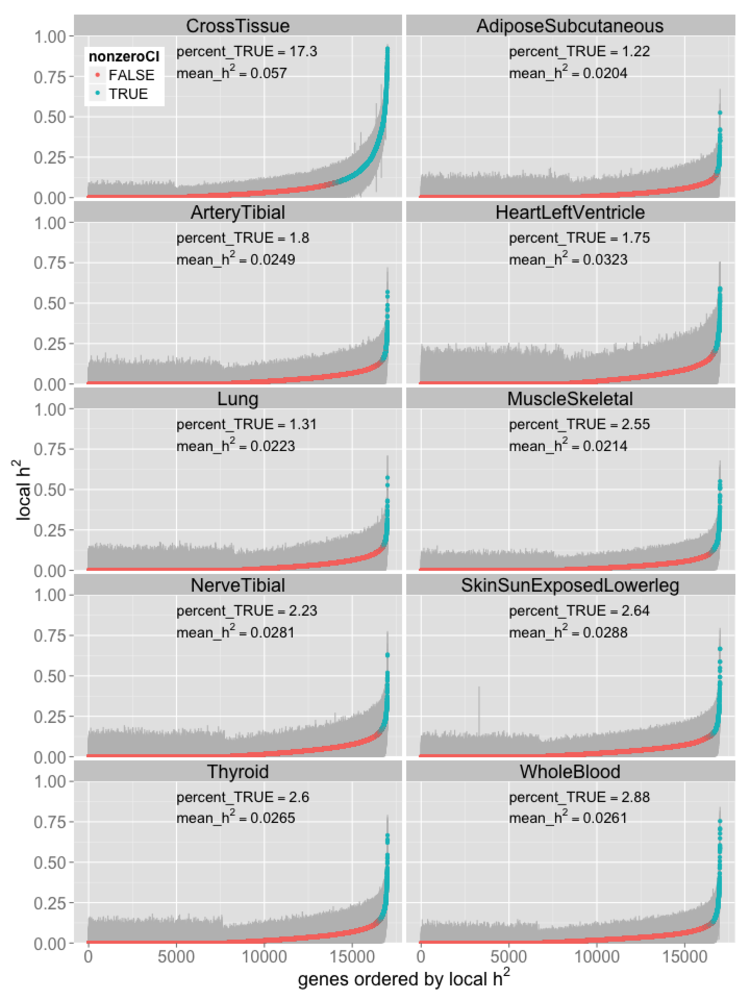
\includegraphics{GenArch_manuscript_files/figure-latex/otdTSh2-1.pdf}
\caption{Cross-tissue heritability (h\textsuperscript{2}) compared to
tissue-specific h\textsuperscript{2}. Cross-tissue local
h\textsuperscript{2} is estimated using the cross-tissue component
(random effects) of the mixed effects model for gene expression and SNPs
within 1 Mb of each gene. Tissue-specifc local h\textsuperscript{2} is
estimated using the tissue-specific component (residuals) of the mixed
effects model for gene expression for each respective tissue and SNPs
within 1 Mb of each gene.}
\end{figure}

\begin{figure}[htbp]
\centering
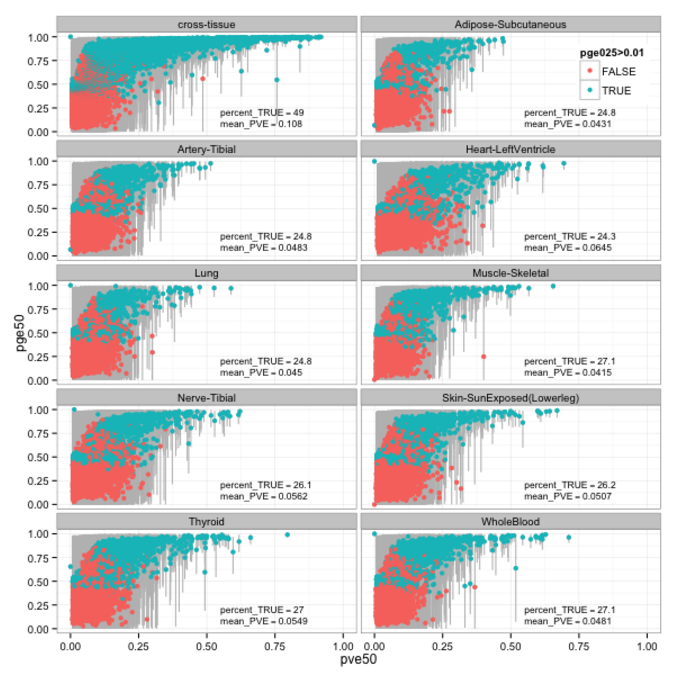
\includegraphics{GenArch_manuscript_files/figure-latex/CTTSbslmm-1.pdf}
\caption{GTEx orthogonal tissue decomposition cross-tissue and
tissue-specific expression comparison of median PGE (proportion of PVE
explained by sparse effects) to median PVE (total proportion of variance
explained) for expression of each gene. The 95\% credible set of each
PGE estimate is in gray and genes with a lower credible set (LCS)
greater than 0.01 are in blue.}
\end{figure}

\begin{figure}[htbp]
\centering
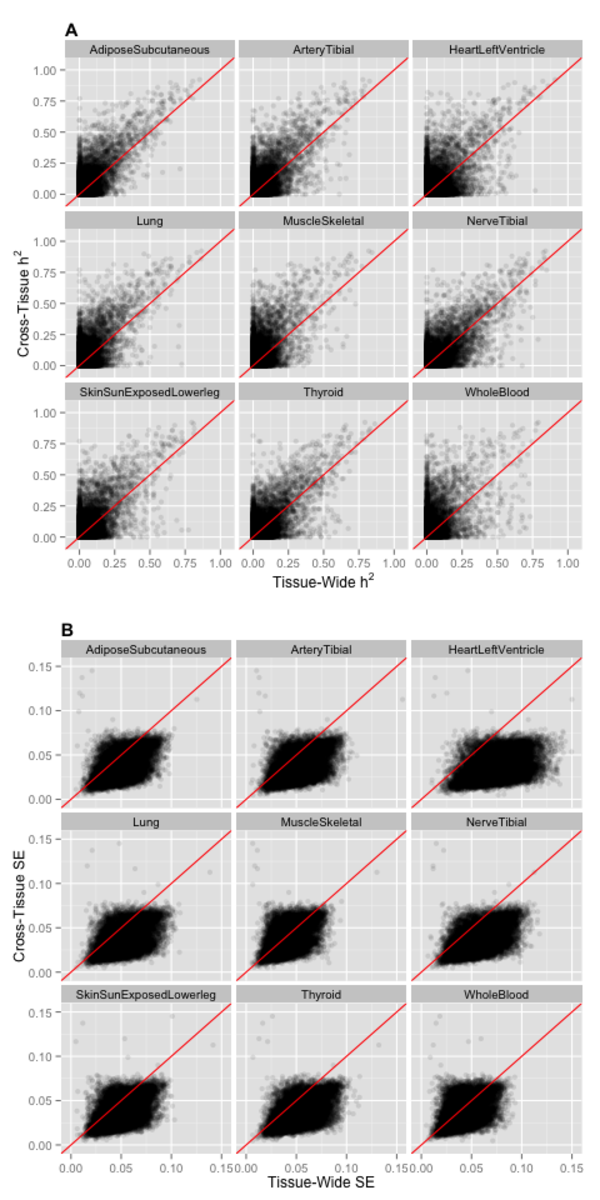
\includegraphics{GenArch_manuscript_files/figure-latex/TWotdH2SE-1.pdf}
\caption{Cross-tissue and whole tissue comparison of heritability
(h\textsuperscript{2}, \textbf{A}) and standard error (SE, \textbf{B}).
Cross-tissue local h\textsuperscript{2} is estimated using the
cross-tissue component (random effects) of the mixed effects model for
gene expression and SNPs within 1 Mb of each gene. Whole tissue local
h\textsuperscript{2} is estimated using the measured gene expression for
each respective tissue and SNPs within 1 Mb of each gene.}
\end{figure}

\begin{figure}[htbp]
\centering
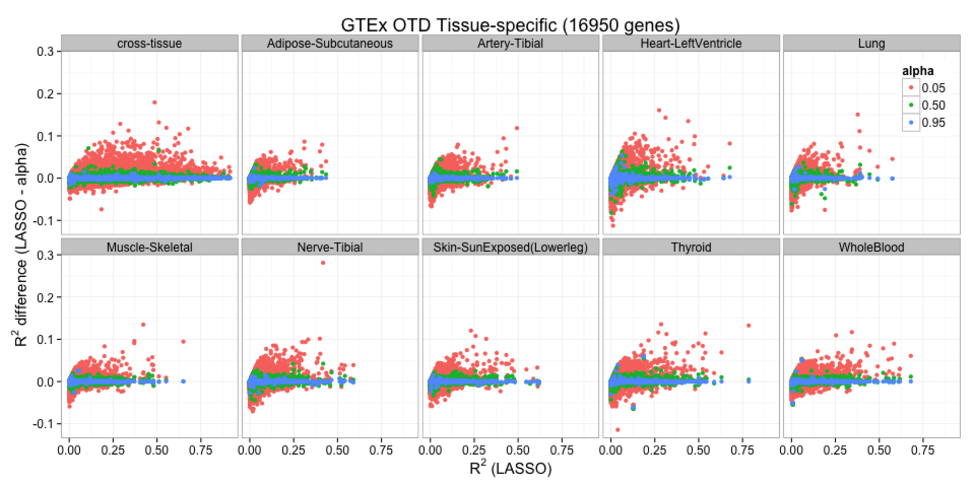
\includegraphics{GenArch_manuscript_files/figure-latex/ENctts-1.pdf}
\caption{GTEx orthogonal tissue decomposition cross-tissue and
tissue-specific expression cross-validated predictive performance across
the elastic net. Predictive R\textsuperscript{2} difference between
LASSO (\(\alpha = 1\)) and several other values of \(\alpha\) compared
to LASSO predictive R\textsuperscript{2} for 18473 autosomal genes per
tissue.}
\end{figure}

\begin{figure}[htbp]
\centering
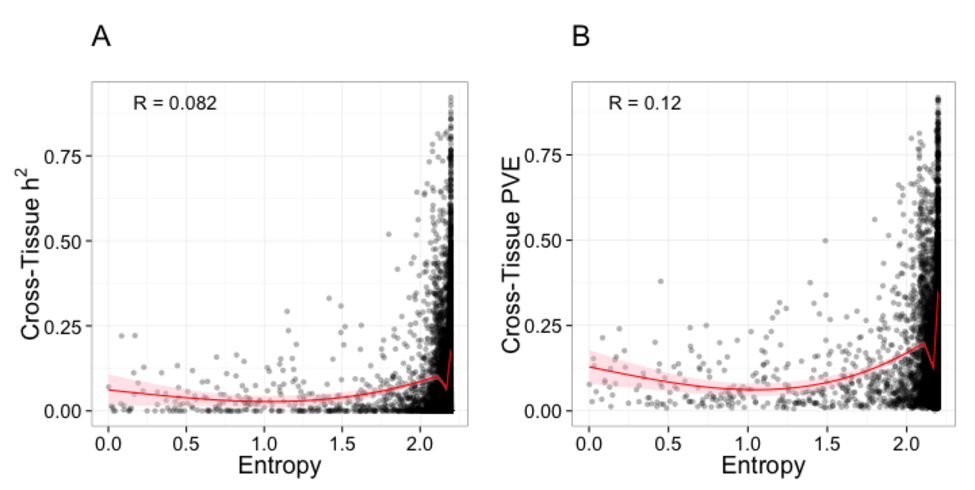
\includegraphics{GenArch_manuscript_files/figure-latex/entropyCT-1.pdf}
\caption{Entropy of the posterior probabilities from the Flutre et al.
multi-tissue eQTL method compared to the estimates of (\textbf{A})
heritability and (\textbf{B}) PVE of cross-tissue gene expression
derived from the orthogonal tissue decomposition. The generalized
additive model smoothing line is in red.}
\end{figure}

\begin{figure}[htbp]
\centering
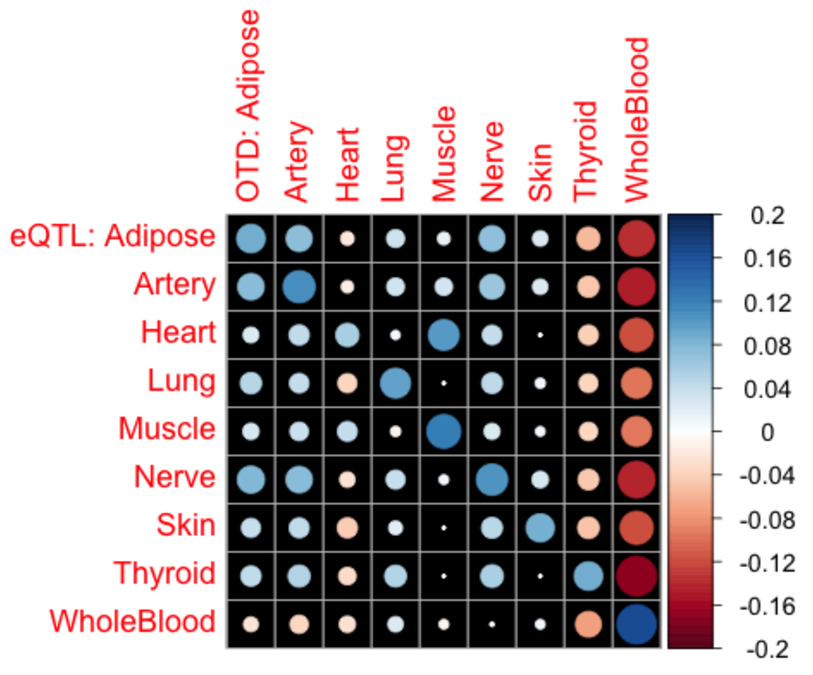
\includegraphics{GenArch_manuscript_files/figure-latex/corrplot-1.pdf}
\caption{Pearson correlation (R) between the posterior probability the
top multi-tissue eQTL regulates its gene in a given tissue (eQTL, Flutre
et al. method) and the PVE of tissue-specific gene expression from the
orthogonal tissue decomposition (OTD). Area of each circle is
proportional to the absolute value of R.}
\end{figure}

\section{Supplemental Figures}\label{supplemental-figures}

\section{Acknowledegments}\label{acknowledegments}

We thank Nicholas Knoblauch and Jason Torres for initial pipeline
development and planning.

\section{Grants}\label{grants}

We acknowledge the following US National Institutes of Health grants:
K12 CA139160 (H.K.I.), T32 MH020065 (K.P.S.), R01 MH101820 and R01
MH090937 (GTEx), P30 DK20595 and P60 DK20595 (Diabetes Research and
Training Center), P50 DA037844 (Rat Genomics), UO1 GM61393
(Pharmacogenomics of Anticancer Agents Research), P50 MH094267 (Conte),
and U19 HL065962 (PGRN Statistical Analysis Resource). H.E.W. was
supported in part by start-up funds from Loyola University Chicago.

\subsection{GTEx data}\label{gtex-data}

The Genotype-Tissue Expression (GTEx) Project was supported by the
Common Fund of the Office of the Director of the National Institutes of
Health (commonfund.nih.gov/GTEx). Additional funds were provided by the
NCI, NHGRI, NHLBI, NIDA, NIMH, and NINDS. Donors were enrolled at
Biospecimen Source Sites funded by NCI Leidos Biomedical Research, Inc.
subcontracts to the National Disease Research Interchange (10XS170),
Roswell Park Cancer Institute (10XS171), and Science Care, Inc.
(X10S172). The Laboratory, Data Analysis, and Coordinating Center
(LDACC) was funded through a contract (HHSN268201000029C) to the The
Broad Institute, Inc. Biorepository operations were funded through a
Leidos Biomedical Research, Inc. subcontract to Van Andel Research
Institute (10ST1035). Additional data repository and project management
were provided by Leidos Biomedical Research, Inc.(HHSN261200800001E).
The Brain Bank was supported supplements to University of Miami grant
DA006227. Statistical Methods development grants were made to the
University of Geneva (MH090941 \& MH101814), the University of Chicago
(MH090951,MH090937, MH101825, \& MH101820), the University of North
Carolina - Chapel Hill (MH090936), North Carolina State University
(MH101819),Harvard University (MH090948), Stanford University
(MH101782), Washington University (MH101810), and to the University of
Pennsylvania (MH101822). The datasets used for the analyses described in
this manuscript were obtained from dbGaP at
\url{http://www.ncbi.nlm.nih.gov/gap} through dbGaP accession number
phs000424.v3.p1.

\subsection{DGN data}\label{dgn-data}

NIMH Study 7 (GenRED I) - Data and biomaterials were collected in six
projects that participated in the National Institute of Mental Health
(NIMH) Genetics of Recurrent Early-Onset Depression (GenRED) project.
From 1999-2003, the Principal Investigators and Co-Investigators were:
New York State Psychiatric Institute, New York, NY, R01 MH060912, Myrna
M. Weissman, Ph.D.~and James K. Knowles, M.D., Ph.D.; University of
Pittsburgh, Pittsburgh, PA, R01 MH060866, George S. Zubenko, M.D.,
Ph.D.~and Wendy N. Zubenko, Ed.D., R.N., C.S.; Johns Hopkins University,
Baltimore, MD, R01 MH059552, J. Raymond DePaulo, M.D., Melvin G.
McInnis, M.D.~and Dean MacKinnon, M.D.; University of Pennsylvania,
Philadelphia, PA, RO1 MH61686, Douglas F. Levinson, M.D. (GenRED
coordinator), Madeleine M. Gladis, Ph.D., Kathleen MurphyEberenz,
Ph.D.~and Peter Holmans, Ph.D. (University of Wales College of
Medicine); this preprint is the author/funder. It is made available
under a CC-BY 4.0 International license. bioRxiv preprint first posted
online June 17, 2015; doi: \url{http://dx.doi.org/10.1101/020164}; The
copyright holder for University of Iowa, Iowa City, IW, R01 MH059542,
Raymond R. Crowe, M.D.~and William H. Coryell, M.D.; Rush University
Medical Center, Chicago, IL, R01 MH059541- 05, William A. Scheftner,
M.D., Rush-Presbyterian. NIMH Study 18 - Data and biomaterials were
obtained from the limited access datasets distributed from the
NIH-supported ``Sequenced Treatment Alternatives to Relieve Depression''
(STAR*D). STAR*D focused on non-psychotic major depressive disorder in
adults seen in outpatient settings. The primary purpose of this research
study was to determine which treatments work best if the first treatment
with medication does not produce an acceptable response. The study was
supported by NIMH Contract \# N01MH90003 to the University of Texas
Southwestern Medical Center. The ClinicalTrials.gov identifier is
NCT00021528. NIMH Study 52 (GenRED II) -- Data and biomaterials in this
release were collected in six projects that participated in the National
Institute of Mental Health (NIMH) Genetics of Recurrent Early-Onset
Depression (GenRED) project (1999-2009). The Principal Investigators and
Co-Investigators were: New York State Psychiatric Institute, New York,
NY, R01 MH 060912, Myrna M. Weissman, Ph.D.; Johns Hopkins University,
Baltimore, MD, R01 MH059552, J. Raymond DePaulo, M.D., and James B.
Potash, M.D., M.P.H.; University of Pennsylvania, Philadelphia, PA
(1999-2005), and Stanford University (2006-2009), R01 MH61686, Douglas
F. Levinson, M.D. (GenRED coordinator); University of Iowa, Iowa City,
IW, R01 MH059542e, Raymond R. Crowe, M.D., and William H. Coryell, M.D.;
Rush University Medical Center, Chicago, IL, R01 MH059541-05, William A.
Scheftner, M.D.; and University of Pittsburgh, Pittsburgh, PA
(1999-2003), R01 MH060866, George S. Zubenko, M.D., Ph.D., and Wendy N.
Zubenko, Ed.D., R.N., C.S. NIMH Study 88 -- Data was provided by
Dr.~Douglas F. Levinson. We gratefully acknowledge the resources were
supported by National Institutes of Health/National Institute of Mental
Health grants 5RC2MH089916 (PI: Douglas F. Levinson, M.D.;
Coinvestigators: Myrna M. Weissman, Ph.D., James B. Potash, M.D., MPH,
Daphne Koller, Ph.D., and Alexander E. Urban, Ph.D.) and 3R01MH090941
(Co-investigator: Daphne Koller, Ph.D.).

\subsection{Computing resources}\label{computing-resources}

This work made use of the Open Science Data Cloud (OSDC) which is an
Open Cloud Consortium (OCC)-sponsored project. This work was supported
in part by grants from Gordon and Betty Moore Foundation and the
National Science Foundation and major contributions from OCC members
like the University of Chicago. this preprint is the author/funder. It
is made available under a CC-BY 4.0 International license. bioRxiv
preprint first posted online June 17, 2015; doi:
\url{http://dx.doi.org/10.1101/020164}; The copyright holder for
\url{https://www.opensciencedatacloud.org/} Grossman RL, Greenway M,
Heath AP, Powell R, Suarez R, Wells W, White KP, Atkinson M, Klampanos
I, Alvarez H, Harvey C and Mambretti J, The Design of a Community
Science Cloud: The Open Science Data Cloud Perspective. (2012)
\url{doi:10.1109/SC.Companion.2012.127} This work made use of the
Bionimbus Protected Data Cloud (PDC), which is a collaboration between
the Open Science Data Cloud (OSDC) and the IGSB (IGSB), the Center for
Research Informatics (CRI), the Institute for Translational Medicine
(ITM), and the University of Chicago Comprehensive Cancer Center
(UCCCC). The Bionimbus PDC is part of the OSDC ecosystem and is funded
as a pilot project by the NIH.
\url{https://www.bionimbus-pdc.opensciencedatacloud.org/} Heath AP,
Greenway M, Powell R, Spring J, Suarez R, Hanley D, Bandlamudi C,
McNerney ME, White KP and Grossman RL, Bionimbus: A Cloud for Managing,
Analyzing and Sharing Large Genomics Datasets. J Am Med Inform Assoc
(2014) \url{doi:10.1136/amiajnl-2013-002155}

\section*{References}\label{references}
\addcontentsline{toc}{section}{References}

1. Nicolae DL, Gamazon E, Zhang W, Duan S, Dolan ME, Cox NJ.
Trait-associated SNPs are more likely to be eQTLs: Annotation to enhance
discovery from GWAS. Gibson G, editor. PLoS Genetics. Public Library of
Science (PLoS); 2010;6: e1000888.
doi:\href{http://dx.doi.org/10.1371/journal.pgen.1000888}{10.1371/journal.pgen.1000888}

2. Nica AC, Montgomery SB, Dimas AS, Stranger BE, Beazley C, Barroso I,
et al. Candidate causal regulatory effects by integration of expression
QTLs with complex trait genetic associations. Gibson G, editor. PLoS
Genetics. Public Library of Science (PLoS); 2010;6: e1000895.
doi:\href{http://dx.doi.org/10.1371/journal.pgen.1000895}{10.1371/journal.pgen.1000895}

3. Gusev A, Lee SH, Trynka G, Finucane H, Vilhj{\a'a}lmsson BJ, Xu H, et
al. Partitioning heritability of regulatory and cell-type-specific
variants across 11 common diseases. The American Journal of Human
Genetics. Elsevier BV; 2014;95: 535--552.
doi:\href{http://dx.doi.org/10.1016/j.ajhg.2014.10.004}{10.1016/j.ajhg.2014.10.004}

4. Purcell SM, Wray NR, Stone JL, Visscher PM, Sullivan MCOPF, Sklar P,
et al. Common polygenic variation contributes to risk of schizophrenia
and bipolar disorder. Nature. Nature Publishing Group; 2009;
doi:\href{http://dx.doi.org/10.1038/nature08185}{10.1038/nature08185}

5. Stahl EA, Wegmann D, Trynka G, Gutierrez-Achury J, Do R, Voight BF,
et al. Bayesian inference analyses of the polygenic architecture of
rheumatoid arthritis. Nature Genetics. Nature Publishing Group; 2012;44:
483--489. doi:\href{http://dx.doi.org/10.1038/ng.2232}{10.1038/ng.2232}

6. Morris AP, Voight BF, Teslovich TM, Ferreira T, Segr{\a`e} AV,
Steinthorsdottir V, et al. Large-scale association analysis provides
insights into the genetic architecture and pathophysiology of type 2
diabetes. Nature Genetics. Nature Publishing Group; 2012;44: 981--990.
doi:\href{http://dx.doi.org/10.1038/ng.2383}{10.1038/ng.2383}

7. Albert FW, Kruglyak L. The role of regulatory variation in complex
traits and disease. Nat Rev Genet. Nature Publishing Group; 2015;16:
197--212. doi:\href{http://dx.doi.org/10.1038/nrg3891}{10.1038/nrg3891}

8. Stranger BE, Montgomery SB, Dimas AS, Parts L, Stegle O, Ingle CE, et
al. Patterns of cis regulatory variation in diverse human populations.
Barsh GS, editor. PLoS Genetics. Public Library of Science (PLoS);
2012;8: e1002639.
doi:\href{http://dx.doi.org/10.1371/journal.pgen.1002639}{10.1371/journal.pgen.1002639}

9. Stranger BE, Nica AC, Forrest MS, Dimas A, Bird CP, Beazley C, et al.
Population genomics of human gene expression. Nature Genetics. Nature
Publishing Group; 2007;39: 1217--1224.
doi:\href{http://dx.doi.org/10.1038/ng2142}{10.1038/ng2142}

10. Innocenti F, Cooper GM, Stanaway IB, Gamazon ER, Smith JD, Mirkov S,
et al. Identification, replication, and functional fine-mapping of
expression quantitative trait loci in primary human liver tissue. Storey
JD, editor. PLoS Genetics. Public Library of Science (PLoS); 2011;7:
e1002078.
doi:\href{http://dx.doi.org/10.1371/journal.pgen.1002078}{10.1371/journal.pgen.1002078}

11. Wright FA, Sullivan PF, Brooks AI, Zou F, Sun W, Xia K, et al.
Heritability and genomics of gene expression in peripheral blood. Nature
Genetics. Nature Publishing Group; 2014;46: 430--437.
doi:\href{http://dx.doi.org/10.1038/ng.2951}{10.1038/ng.2951}

12. Price AL, Helgason A, Thorleifsson G, McCarroll SA, Kong A,
Stefansson K. Single-tissue and cross-tissue heritability of gene
expression via identity-by-descent in related or unrelated individuals.
Gibson G, editor. PLoS Genetics. Public Library of Science (PLoS);
2011;7: e1001317.
doi:\href{http://dx.doi.org/10.1371/journal.pgen.1001317}{10.1371/journal.pgen.1001317}

13. Gamazon ER, Wheeler HE, Shah KP, Mozaffari SV, Aquino-Michaels K,
Carroll RJ, et al. A gene-based association method for mapping traits
using reference transcriptome data. Nature Genetics. Nature Publishing
Group; 2015;47: 1091--1098.
doi:\href{http://dx.doi.org/10.1038/ng.3367}{10.1038/ng.3367}

14. Regression shrinkage and selection via the lasso on jSTOR
{[}Internet{]}. \url{http://www.jstor.org/stable/2346178}; 2015.
Available: \url{http://www.jstor.org/stable/2346178}

15. Hoerl AE, Kennard RW. Ridge regression: Applications to
nonorthogonal problems. Technometrics. Informa UK Limited; 1970;12:
69--82.
doi:\href{http://dx.doi.org/10.1080/00401706.1970.10488635}{10.1080/00401706.1970.10488635}

16. {de los Campos} G, Gianola D, Allison DB. Predicting genetic
predisposition in humans: The promise of whole-genome markers. Nat Rev
Genet. Nature Publishing Group; 2010;11: 880--886.
doi:\href{http://dx.doi.org/10.1038/nrg2898}{10.1038/nrg2898}

17. Wheeler HE, Aquino-Michaels K, Gamazon ER, Trubetskoy VV, Dolan ME,
Huang RS, et al. Poly-omic prediction of complex traits: OmicKriging.
Genetic Epidemiology. Wiley-Blackwell; 2014;38: 402--415.
doi:\href{http://dx.doi.org/10.1002/gepi.21808}{10.1002/gepi.21808}

18. Zhou X, Carbonetto P, Stephens M. Polygenic modeling with bayesian
sparse linear mixed models. Visscher PM, editor. PLoS Genetics. Public
Library of Science (PLoS); 2013;9: e1003264.
doi:\href{http://dx.doi.org/10.1371/journal.pgen.1003264}{10.1371/journal.pgen.1003264}

19. Cheung VG, Spielman RS, Ewens KG, Weber TM, Morley M, Burdick JT.
Mapping determinants of human gene expression by regional and
genome-wide association. Nature. Nature Publishing Group; 2005;437:
1365--1369.
doi:\href{http://dx.doi.org/10.1038/nature04244}{10.1038/nature04244}

20. Battle A, Mostafavi S, Zhu X, Potash JB, Weissman MM, McCormick C,
et al. Characterizing the genetic basis of transcriptome diversity
through RNA-sequencing of 922 individuals. Genome Research. Cold Spring
Harbor Laboratory Press; 2013;24: 14--24.
doi:\href{http://dx.doi.org/10.1101/gr.155192.113}{10.1101/gr.155192.113}

21. Ardlie KG, Deluca DS, Segre AV, Sullivan TJ, Young TR, Gelfand ET,
et al. The genotype-tissue expression (GTEx) pilot analysis: Multitissue
gene regulation in humans. Science. American Association for the
Advancement of Science (AAAS); 2015;348: 648--660.
doi:\href{http://dx.doi.org/10.1126/science.1262110}{10.1126/science.1262110}

22. Yang J, Lee SH, Goddard ME, Visscher PM. GCTA: A tool for
genome-wide complex trait analysis. The American Journal of Human
Genetics. Elsevier BV; 2011;88: 76--82.
doi:\href{http://dx.doi.org/10.1016/j.ajhg.2010.11.011}{10.1016/j.ajhg.2010.11.011}

23. Zhang X, Joehanes R, Chen BH, Huan T, Ying S, Munson PJ, et al.
Identification of common genetic variants controlling transcript isoform
variation in human whole blood. Nature Genetics. Nature Publishing
Group; 2015;47: 345--352.
doi:\href{http://dx.doi.org/10.1038/ng.3220}{10.1038/ng.3220}

24. Zou H, Hastie T. Regularization and variable selection via the
elastic net. Journal of the Royal Statistical Society: Series B
(Statistical Methodology). Wiley-Blackwell; 2005;67: 301--320.
doi:\href{http://dx.doi.org/10.1111/j.1467-9868.2005.00503.x}{10.1111/j.1467-9868.2005.00503.x}

25. Flutre T, Wen X, Pritchard J, Stephens M. A statistical framework
for joint eQTL analysis in multiple tissues. Gibson G, editor. PLoS
Genetics. Public Library of Science (PLoS); 2013;9: e1003486.
doi:\href{http://dx.doi.org/10.1371/journal.pgen.1003486}{10.1371/journal.pgen.1003486}

26. Hemani G, Yang J, Vinkhuyzen A, Powell JE, Willemsen G, Hottenga
J-J, et al. Inference of the genetic architecture underlying BMI and
height with the use of 20,240 sibling pairs. The American Journal of
Human Genetics. Elsevier BV; 2013;93: 865--875.
doi:\href{http://dx.doi.org/10.1016/j.ajhg.2013.10.005}{10.1016/j.ajhg.2013.10.005}

27. Howie B, Fuchsberger C, Stephens M, Marchini J, Abecasis GR. Fast
and accurate genotype imputation in genome-wide association studies
through pre-phasing. Nature Genetics. Nature Publishing Group; 2012;44:
955--959. doi:\href{http://dx.doi.org/10.1038/ng.2354}{10.1038/ng.2354}

28. Fuchsberger C, Abecasis GR, Hinds DA. Minimac2: Faster genotype
imputation. Bioinformatics. Oxford University Press (OUP); 2014;31:
782--784.
doi:\href{http://dx.doi.org/10.1093/bioinformatics/btu704}{10.1093/bioinformatics/btu704}

29. Harrow J, Frankish A, Gonzalez JM, Tapanari E, Diekhans M,
Kokocinski F, et al. GENCODE: The reference human genome annotation for
the ENCODE project. Genome Research. Cold Spring Harbor Laboratory
Press; 2012;22: 1760--1774.
doi:\href{http://dx.doi.org/10.1101/gr.135350.111}{10.1101/gr.135350.111}

30. Friedman J, Hastie T, Tibshirani R. Regularization paths for
generalized linear models via coordinate descent. Journal of Statistical
Software. 2010;33: 1--22. Available:
\url{http://www.jstatsoft.org/v33/i01/}

31. Simon N, Friedman J, Hastie T, Tibshirani R. Regularization paths
for cox's proportional hazards model via coordinate descent. Journal of
Statistical Software. 2011;39: 1--13. Available:
\url{http://www.jstatsoft.org/v39/i05/}

32. Zhou X, Stephens M. Genome-wide efficient mixed-model analysis for
association studies. Nature Genetics. Nature Publishing Group; 2012;44:
821--824. doi:\href{http://dx.doi.org/10.1038/ng.2310}{10.1038/ng.2310}

33. Im HK, Gamazon ER, Stark AL, Huang RS, Cox NJ, Dolan ME. Mixed
effects modeling of proliferation rates in cell-based models:
Consequence for pharmacogenomics and cancer. Akey JM, editor. PLoS
Genetics. Public Library of Science (PLoS); 2012;8: e1002525.
doi:\href{http://dx.doi.org/10.1371/journal.pgen.1002525}{10.1371/journal.pgen.1002525}

34. R Core Team. R: A language and environment for statistical computing
{[}Internet{]}. Vienna, Austria: R Foundation for Statistical Computing;
2015. Available: \url{http://www.R-project.org/}

35. Bates D, Maechler M, Bolker B, Walker S. lme4: Linear mixed-effects
models using Eigen and S4 {[}Internet{]}. 2015. Available:
\url{http://CRAN.R-project.org/package=lme4}

36. Bates D, Maechler M, Bolker BM, Walker S. Fitting linear
mixed-effects models using lme4 {[}Internet{]}. 2015. Available:
\url{http://arxiv.org/abs/1406.5823}

37. Stegle O, Parts L, Piipari M, Winn J, Durbin R. Using probabilistic
estimation of expression residuals (PEER) to obtain increased power and
interpretability of gene expression analyses. Nat Protoc. Nature
Publishing Group; 2012;7: 500--507.
doi:\href{http://dx.doi.org/10.1038/nprot.2011.457}{10.1038/nprot.2011.457}

\end{document}
